\documentclass[tikz]{standalone}
\usepackage{tikz}
\begin{document}
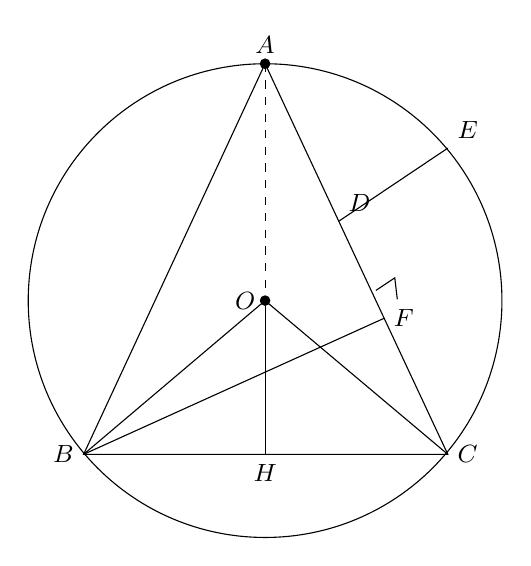
\begin{tikzpicture}[scale=1.6, font=\small,
  pt/.style={circle, fill=black, inner sep=0.9pt}]

% Circumcircle (center O, radius ~1.88)
\coordinate (A) at (2.17,-0.65);
\coordinate (B) at (0.73,-3.75);
\coordinate (C) at (3.62,-3.75);
\coordinate (H) at (2.17,-3.75);
\coordinate (O) at (2.17,-2.53);
\coordinate (D) at (2.755,-1.90);
\coordinate (E) at (3.62,-1.32);
\coordinate (F) at (3.115,-2.67);

\draw (O) circle (1.88);

% Triangle sides
\draw (A) -- (B) -- (C) -- cycle;

% Altitude AH (dashed above O, solid below O)
\draw[dashed] (A) -- (O);
\draw (O) -- (H);

% Segments from O and from B
\draw (O) -- (B);
\draw (O) -- (C);
\draw (B) -- (F);

% Line through O, D, E: only the part D--E is kept (segment DO removed)
\draw (D) -- (E);

% Right angle mark near F
\draw (3.05,-2.45) -- (3.20,-2.35) -- (3.22,-2.52);

% Points
\fill (A) circle (1.2pt);
\fill (O) circle (1.2pt);

% Labels
\node[above] at (A) {$A$};
\node[left]  at (B) {$B$};
\node[right] at (C) {$C$};
\node[below] at (H) {$H$};
\node[left]  at (O) {$O$};
\node[above right] at (D) {$D$};
\node[above right] at (E) {$E$};
\node[right] at (F) {$F$};

\end{tikzpicture}
\end{document}
